\Chapter{Implementatie\label{hfdst-implementatie}}

In dit hoofdstuk wordt de implementatie van een schakeling voor de berekening van de Tate pairing uit de doeken gedaan. Het uiteindelijke doel is een compacte ASIC implementatie te verkrijgen.

Er zal onderzocht worden welke basisbewerkingen nodig zijn en hoe deze verwezenlijkt kunnen worden in hardware. Vervolgens wordt een schakeling ontworpen die aan de hand hiervan alle nodige berekeningen kan uitvoeren in het gekozen veld. Ten slotte is er dan nog de schakeling die alle berekeningen voor het Miller algoritme (zie \refsect{sectie-pairings-miller}) in goede banen leidt. In het volgende hoofdstuk zal de resulterende schakeling dan beoordeeld worden.

Allereerst worden echter noodzakelijke parameters vastgelegd, zodat alle bewerkingen exact gedefini\"eerd kunnen worden. Vervolgens wordt bekeken welke beperkingen aan de schakeling opgelegd moeten worden.

\section{Parameters\label{sectie-implementatie-parameters}}

Alvorens kan begonnen worden met de implementatie, moeten bepaalde parameters vastgelegd worden. Pas eens dat gedaan is, zijn alle bewerkingen volledig gedefinieerd.

Een belangrijke parameter is de kromme en het veld waarover gewerkt zal worden. Omdat de berekeningen in een veld $\mathbb{F}_2$ (en extensies ervan) veel eenvoudiger zijn dan die in een veld modulo een priemgetal, wordt ervoor gekozen in zulk een veld te werken.
Verder wordt gekozen voor een supersingulaire elliptische kromme. Dat type krommen heeft een kleine embedding degree en er bestaan simpele rekenregels voor de verdubbeling en optelling van punten. De vergelijking van zo een kromme $E$ over een veld $\mathbb{F}_{2^m}$ wordt gegeven door
\[E: y^3 + y = x^3 + x + b,\]
waarbij $b \in \{0, 1\}$. De embedding degree $k = 4$ voor dit type krommen. Verder worden de volgende hulp variabelen bepaald:
\[\begin{aligned}
\delta	&= b	\qquad	& m \equiv 1, 7 (\bmod 8)\\
			&= 1 - b		& m \equiv 3, 5 (\bmod 8)\\
\nu		&= (-1)^{\delta}\\
\end{aligned}\]
De orde van de kromme is gelijk aan \cite{bertoni, beuchat}:
\[\begin{aligned}
\#E(\mathbb{F}_{2^m})	&= 2^m + \nu \sqrt{2^{m + 1}} + 1
\end{aligned}\]
Om de Tate pairing te kunnen berekenen, moet de variabele $b$ zo gekozen worden dat $\#E$ enkel uit sommaties bestaat. Met andere woorden: $b$ moet zo gekozen worden dat $\nu = 1$.

Alvorens dit kan gebeuren, moet een woordlengte $m$ vastgelegd worden. Deze bepaald de cryptografische sterkte alsook de grootte van het eindresultaat. Des te groter $m$, des te groter de benodigde registers om alle data in op te slaan. In \reftbl{tabel-implementatie-parameters-keylength} zijn enkele vaak gebruikte woordlengtes voor pairings met hun bijhorende sterkte terug te vinden. Er wordt gekozen voor $m = 163$. Dit laat een mooi compromis toe tussen cryptografische sterkte en compactheid van de implementatie.

\begin{table}[h]
	\caption{Vergelijking van woordlengtes $m$ en de bijhorende cryptografische sterkte van de Tate pairing}
	\label{tabel-implementatie-parameters-keylength}

	\centering
	\begin{tabular}{|l|l|}
		\hline
		$m$ (bit)	& sterkte (bit)\\
		\hline
		81		& 324\\
		163	& 652\\
		239	& 956\\
		\hline		
	\end{tabular}
\end{table}

Nu $m$ vastgelegd is, kan hetzelfde gedaan worden voor $b$. Om een aftrekking in de formule voor $\#E$ te voorkomen, dient $b = 1$ te zijn in dit geval. Meteen kan dan ook een $l$-torsiepunt subgroep over $E$ vastgelegd worden. Daarbij moet er op gelet worden dat $l \mid \#E$. De eenvoudigste keuze is:
\[\begin{aligned}
l	&= \#E = 2^{163} + \sqrt{2^{163 + 1}} + 1\\
	&= 2^{163} + 2^{82} + 1.\\
\end{aligned}\]

Nu het veld waarover gewerkt wordt, bepaald is, kan een reductie veelterm $P$ gekozen worden. Bij de keuze daarvan werd uitgegaan van de aangeraden parameters in \cite{sec2}. De veelterm is:
\[P = z^{163} + z^7 + z^6 + z^3 + 1.\]

Ook moet het extensieveld $\mathbb{F}_{2^{k m}}$ gedefinieerd worden waarover de Tate pairing berekend zal worden. Aangezien $k = 4$, kan het veld opgebouwd worden in twee stappen. Eerst wordt $\mathbb{F}_{2^{2m}}$ bepaald als volgt:
\[\mathbb{F}_{2^{2m}} \cong \mathbb{F}_{2^m}[x]/(x^2 + x ^ 1)\]
en hierop wordt het volgende extensieveld gebouwd:
\[\mathbb{F}_{2^{4m}} \cong \mathbb{F}_{2^{2m}}[y]/(y^2 + (x + 1)y + 1).\]
Een element van $\mathbb{F}_{2^{4m}}$ kan dus voorgesteld worden als vier elementen van $\mathbb{F}_{2^m}$.

Ten slotte moet een distortiemap voor gebruik in de berekening van de Tate bepaald worden. Hiervoor wordt dezelfde gekozen als in \cite{bertoni}. Een punt $A \in \mathbb{F}_{2^m}$ ondergaat onder de distortie volgende transformatie:
\[\phi : (x_A, y_A) \to (x_A + s^2, y_A + x_A s + t^6)\]
met $s, t \in \mathbb{F}_{2^{4m}}$. Verder moeten $s$ en $t$ voldoen aan volgende vergelijkingen:
\[\begin{gathered}
s^4 + s = 0\\
t^2 + t + s^6 + s^2 = 0.
\end{gathered}\]
Een mogelijke oplossing hiervoor is:
\[\begin{aligned}
s	&= x + 1\\
t	&= xy.
\end{aligned}\]
Een distortie van $A$ kan dus ook geschreven worden als:
\[\begin{aligned}
x_\phi	&= x_A + x\\
y_\phi	&= (x_A + y_A) + x_A \cdot x + xy.
\end{aligned}\]
Merk op dat de co\"effici\"ent van $1$ van $x_\phi$ en die van $x$ van $y_\phi$ beiden gelijk zijn aan $x_A$. Door deze handige vorm zullen in de implementatie slechts twee registers nodig zijn om de distortie van het punt $Q$ bij te houden.

\section{Beperkingen\label{sectie-implementatie-beperkingen}}

Het doel is de uiteindelijke schakeling zo klein mogelijk te maken, zodat ze gebruikt kan worden in bv.\ netwerken van sensoren of een smartcard. Beperking van de oppervlakte is dus de belangrijkste factor. Een tweede belangrijke factor is vermogenverbruik, om dit te beperken bestaan specifieke technieken. Het verbruik hangt ook samen met de oppervlakte, dus het beperken daarvan zal het verbruik ten goede komen. In eerste instantie zal dus getracht worden de implementatie zo compact mogelijk te maken. Het verbruik kan verder ook verlaagd worden door een lagere kloksnelheid voor de schakeling te gebruiken, wat uiteraard de rekensnelheid niet bevordert. De rekensnelheid is echter geen prioriteit en dus zal dit aspect bij het ontwerp van de schakelingen genegeerd worden.

Algemeen kan dus gesteld worden dat hoe kleiner het uiteindelijke resultaat is, hoe beter. Het is dus cruciaal de elementen te identificeren die het meeste plaats innemen in een ASIC schakeling. In \reftbl{tabel-implementatie-beperkingen-elementen-gatecount} is de grootte van de belangrijkste elementen te vinden. Deze cijfers gelden enkel bij gebruik van $0.13 \mu m$ low leakage technologie van Faraday Technology Corporation. De ordening van de elementen zal echter grotendeels behouden voor andere technologi\"en. Uit de tabel blijkt dat het gebruik van flip-flops (registers), adders en multiplexers zoveel mogelijk beperkt moet worden.

\begin{table}[h]
	\caption[Grootte van elementen in een ASIC schakeling in gates$/$bit ($0.13 \mu m$ low leakage technologie van Faraday Technology Corporation)]{Grootte van elementen in een ASIC schakeling in gates$/$bit ($0.13 \mu m$ low leakage technologie van Faraday Technology Corporation) \cite{cell-databook}}
	\label{tabel-implementatie-beperkingen-elementen-gatecount}

	\centering
	\begin{tabular}{|l|r|}
		\hline
		Element			& Gates$/$bit\\
		\hline
		D flip-flop met reset	& 6\\
		D flip-flop zonder reset	& 5.5\\
		full adder		& 5.5\\
		D latch			& 4.25\\
		3 ingang MUX	& 4\\
		2 ingang XNOR	& 3.75\\
		2 ingang XOR	& 3.75\\
		2 ingang MUX	& 2.25\\
		2 ingang OR		& 1.25\\
		2 ingang AND	& 1.25\\
		2 ingang NOR	& 1\\
		2 ingang NAND	& 1\\
		NOT				& 0.75\\
		\hline		
	\end{tabular}
\end{table}

\section{Modular Arithmetic Logical Unit\label{sectie-implementatie-malu}}

De kern van de hardware implementatie wordt gevormd door de Modular Arithmetic Logical Unit (MALU) \cite{sakiyama, batina-lowcost}. Dit circuit laat toe basis bewerkingen uit te voeren op getallen. Gezien de beperking die is opgelegd aan de oppervlakte van de schakeling, wordt enkel de optelling ge\"implementeerd. Later wordt met behulp daarvan elke andere nodige berekening verwezenlijkt.

Aangezien er in het veld $\mathbb{F}_{2^m}$ gewerkt wordt, is een optelling equivalent aan een XOR bewerking. De bewerking die moet uitgevoerd kunnen worden is:

\[\begin{aligned}
T + B	&= T \xor B\\
		&= R \mod P
\end{aligned}\]

Merk op dat bij een optelling de graad van $R$ enkel kleiner of gelijk kan zijn aan die van $T$ en $B$. Indien $B$ van graad $< m$ is (dus $\in \mathbb{F}_{2^m}$) en $T$ van graad $\leq m$ ($\in \mathbb{F}_{2^{m+1}}$), is de optelling te implementeren als in \refalg{algoritme-implementatie-malu-modulo}.

\begin{algorithm}[h]
	\caption{Modulo optelling in $\mathbb{F}_{2^m}$}
	\label{algoritme-implementatie-malu-modulo}
	\KwIn{$B \in \mathbb{F}_{2^m}$, $T \in \mathbb{F}_{2^{m + 1}}$}
	\KwOut{$R \mod P \in \mathbb{F}_{2^m}$}
	\SetKwFunction{Degree}{Degree}

	$R \leftarrow T \xor B$\;

	\If{$\Degree{R} = m$}{
		$R \leftarrow R \xor P$\;
	}
\end{algorithm}

In \refsect{sectie-implementatie-miller-forlus} zal blijken dat het vaak nodig zal zijn om het resultaat $R$ te vermenigvuldigen met $z$, m.a.w.\ alle bits 1 plaats naar links te verschuiven. Een voor de hand liggende schakeling die dit alles implementeert, is te zien in \reffig{figuur-implementatie-malu-basic}. Ingang $P_{\text{in}}$ dient afhankelijk van de graad van $T$ ingesteld te worden op $0$ of $P$. De ingangen $T$ en $P_{\text{in}}$ zijn $m$ bits aangezien het resultaat voor de vermenigvuldiging met $z$ steeds van graad $< m$ is en bit $m + 1$ dus toch steeds 0 zou zijn. De hoogste graad term na de shift wordt naar buiten gebracht als $mod_{\text{u}}$. De implementatie bestaat uit $2m$ XOR poorten.

\begin{figure}[h]
	\centering
		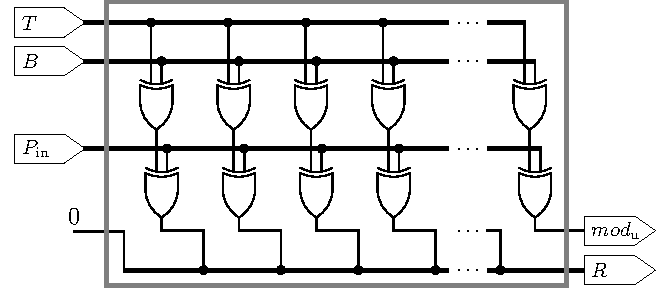
\includegraphics[width=12cm]{malu-basic}
		\caption{MALU - Basis ontwerp met shift\label{figuur-implementatie-malu-basic}}
\end{figure}

Aangezien voor het ontwerp het veld en de modulo veelterm op voorhand bepaald zijn, is het mogelijk een zeer groot aantal XOR poorten uit het ontwerp te verwijderen. De ingang $P$ en de bijhorende $m$ XOR poorten kunnen vervangen worden door een 1 bit `modulo enable' ingang $mod_{\text{e}}$ en er worden enkel XOR poorten geplaatst voor de bits $i$ waarvoor $P_i = 1$. Hierdoor wordt het aantal ingangen drastisch verkleind en worden 
\[\Delta = m - (\textsf{Hamm}(P) - 1)\]
XOR poorten uitgespaard, met \textsf{Hamm}$(P)$ gelijk aan het Hamming gewicht van de binaire representatie van $P$.

In dit geval is $m = 163$ en $P = z^{163} + z^7 + z^6 + z^3 + 1$. Er zijn dus $\textsf{Hamm}(P) - 1 = 4$ XOR poorten nodig, wat een besparing van $163 - 4 =  159$ XOR poorten oplevert ($51\%$ minder dan het oorsponkelijk aantal).

De resulterende schakeling is te zien in \reffig{figuur-implementatie-malu-optimized}.

\begin{figure}[h]
	\centering
		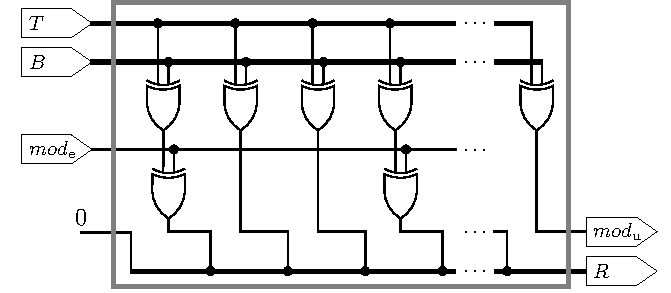
\includegraphics[width=12cm]{malu-optimized}
		\caption{MALU - Geoptimaliseerd ontwerp met shift\label{figuur-implementatie-malu-optimized}}
\end{figure}

\section{Berekeningen in $\mathbb{F}_{2^m}$\label{sectie-implementatie-gf2m}}

\subsection{Basisontwerp\label{subsectie-implementatie-gf2m-basisontwerp}}

De eerder ontworpen MALU schakeling laat toe optellingen te doen, maar het Miller algoritme vereist dat er ook vermenigvuldigingen worden uitgerekend. Delingen en machtsverheffingen kunnen met behulp van vermenigvuldiging berekend worden en dienen dus niet rechtstreeks ge\"implementeerd te worden. Indien dus zowel optellingen als vermenigvuldigingen berekend kunnen worden, is alles voorhanden om de Tate pairing te berekenen.

Door toepassing van een ``shift and add'' algoritme, kan de waarde van \mbox{$A \cdot B = R$} berekend worden met behulp van de MALU schakeling. In \refalg{algoritme-implementatie-gf2m-multiply} is te zien hoe dit juist in z'n werk gaat. Door de modulo operatie telkens op het tussenresultaat uit te voeren, is het steeds van graad $\leq m$ en kan het opgeslagen worden in $T$. Op het einde moet het resultaat door $z$ gedeeld worden, wat neerkomt op een verschuiving van alle bits met 1 plaats naar rechts.

\begin{algorithm}[h]
	\caption{``Shift and add'' vermenigvuldiging in $\mathbb{F}_{2^m}$}
	\label{algoritme-implementatie-gf2m-multiply}
	\KwIn{$A, B \in \mathbb{F}_{2^m}$}
	\KwOut{$R = A \cdot B \in \mathbb{F}_{2^m}$}
	\KwData{$T \in \mathbb{F}_{2^{m + 1}}$}
	\SetKwFunction{Degree}{Degree}

	$T \leftarrow 0$\;
	\For{$i \leftarrow m - 1$ \KwTo $0$}{
		\eIf{$A_i = 1$}{
			$b \leftarrow B$\;
		}{
			$b \leftarrow 0$\;
		}
	
		$T \leftarrow T \xor b$\;
	
		\If{$\Degree{T} = m$}{
			$T \leftarrow T \xor P$\;
		}
		$T \leftarrow T \ll 1$\;
	}
	$R \leftarrow T \gg 1$\;
\end{algorithm}

Wanneer de optelling en vermenigvuldiging nu in een schakeling gegoten worden, dient te schakeling te weten welke van de twee bewerkingen moet uitgevoerd worden. Verder moet het mogelijk zijn de uitkomt $R$ in het register $T$ op te slaan. Op die manier is het mogelijk de uitgang van de schakeling gelijk te stellen aan $R$ zolang geen nieuwe berekening gestart wordt.  

Verderop zal gezien worden dat in het Miller algoritme verscheidene keren de som $R + 1$ moet berekend worden. Daarom wordt aan de schakeling een ingang $plus\_one$ toegevoegd die hierin helpt voorzien. De uiteindelijke schakeling is te zien in \reffig{figuur-implementatie-wrapper-gf2m}. Er wordt zo veel mogelijk bespaard op registers. Het register $cycle$ (equivalent aan $i$ in \refalg{algoritme-implementatie-gf2m-multiply}) is $\lceil \log _2 (m) \rceil$ bits lang en register $T$ $m$ bits. De waarde van $T_m$ wordt opgeslagen in register $mod$. Alle overige registers zijn 1 bit groot. Merk dus op dat de variabele $T$ uit \refalg{algoritme-implementatie-gf2m-multiply} hier gevormd wordt door de combinatie van de registers $T$ en $mod$. 

Voor $A$ wordt geen appart register voorzien en in plaats van $A_i$ wordt steeds bit $A_m$ ingelezen voor de vermenigvuldiging. De schakeling die van deze schakeling gebruik maakt, dient dus te voorzien in een methode om elke klokslag de juiste $A_i$ aan te bieden op $A_m$. Dit kan simpelweg gebeuren door elke klokslag na de start van de berekening het register dat $A$ bevat \'e\'en positie naar links door te schuiven.

\begin{figure}[h]
	\centering
		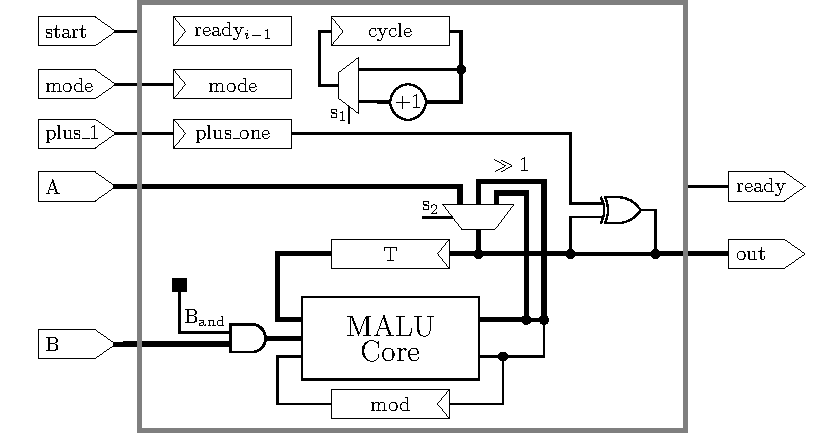
\includegraphics[width=12cm]{wrapper-gf2m}
		\caption{Schakeling voor berekeningen in $\mathbb{F}_{2^m}$\label{figuur-implementatie-wrapper-gf2m}}
\end{figure}

Gezien de eenvoud van de schakeling is het niet nodig een FSM te implementeren, de besturing kan volledig via logica gebeuren. Die wordt getoond in \reffig{figuur-implementatie-wrapper-gf2m-logica}. De werking is zeer eenvoudig: zo lang $start$ hoog is, worden de registers $mode$ en $plus\_one$ geladen met hun respectievelijke ingangen. Verder wordt, afhankelijk van $mode$, $F$ ingeladen met de waarde van $A$ (optelling, $mode = 0$) of gelijkgesteld aan nul (vermenigvuldiging, $mode = 1$). Ook wordt $cycle$ gereset. Wanneer $start$ laag is, wordt, afhankelijk van de gewenste bewerking en de waarde van $ready$, het register $T$ geladen met de uitgang $R$ van de MALU of het uiteindelijke resultaat $R_{\text{ready}} = R \gg 1$.

\begin{figure}[h]
	\centering
		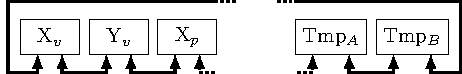
\includegraphics[width=12cm]{wrapper-gf2m-logica}
		\caption{Logica voor besturing van de schakeling voor berekeningen in $\mathbb{F}_{2^m}$\label{figuur-implementatie-wrapper-gf2m-logica}}
\end{figure}

\subsection{Versnelling van de vermenigvuldiging\label{subsectie-implementatie-gf2m-versnelling}}

Wanneer met behulp van de schakeling in \reffig{figuur-implementatie-wrapper-gf2m} een vermenigvuldiging wordt berekend, zal het $m$ klokcycli duren eer het resultaat beschikbaar is aan de uitgang. Het is echter mogelijk dat aantal drastisch naar beneden te halen door $d$ MALU's te gebruiken en dus $d$ optellingen per klokcyclus uit te voeren. Het principe hiervan wordt ge\"illustreerd in \reffig{figuur-implementatie-wrapper-gf2m-d}.

\begin{figure}[h]
	\centering
		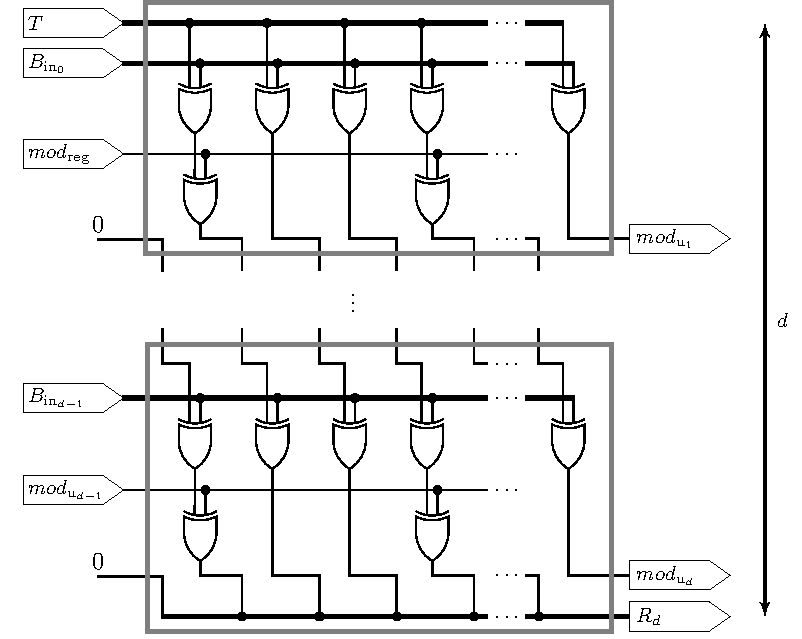
\includegraphics[width=12cm]{malu-width-d}
		\caption{Schakeling voor berekeningen in $\mathbb{F}_{2^m}$ met woordbreedte $d$\label{figuur-implementatie-wrapper-gf2m-d}}
\end{figure}

De rekentijd van het Miller algoritme zal door toepassing van deze techniek gevoelig verkort kunnen worden. Hoe groter $m$ en hoe meer vermenigvuldigigen er uitgevoerd dienen te worden, des te significanter de tijdswinst die geboekt kan worden. Uiteraard gaat het gebruik van deze techniek wel in tegen de eerder opgelegde beperking aan de grootte van de uiteindelijke schakeling. Het is echter niet zo dat er enkel $d - 1$ extra MALU blokken dienen toegevoegd te worden, afhankelijk van $d$ en $m$ dient ook een extra multiplexer in de schakeling gestoken te worden. Dit is zoals opgemerkt in \refsect{sectie-implementatie-beperkingen} een zeer slechte zaak voor de  oppervlakte.

Stel bijvoorbeeld $d = 4$ (en $m = 	163$). Het resultaat van een optelling zal net zoals in het standaard ontwerp (\reffig{figuur-implementatie-wrapper-gf2m}) aanwezig zijn aan de uitgang van MALU \nr 1. Het resultaat van een vermenigvuldiging zal echter aan de uitgang van MALU \nr 3 verschijnen, aangezien $163 \bmod 4 = 3$. Het eindresultaat dat in register $T$ dient opgeslagen te worden, is voor een vermenigvuldiging dus
\[R_{3_{\text{ready}}} = mod{\text{u}_3} \text{ \# } R_{3_{162:1}},\]
terwijl dit voor een optelling
\[R_{1_{\text{ready}}} = mod_{\text{u}_1} \text{ \# } R_{1_{162:1}}\]
is. Met andere woorden, er dient nu niet enkel gekozen te kunnen worden tussen de ingangen $A$, $R_d$ of $R_{1_{\text{ready}}}$, maar ook voor $R_{3_{\text{ready}}}$.

Indien men toch wenst het vermenigvuldigen te versnellen, is het aangeraden een $d$ te kiezen waarvoor $m \bmod d = 1$. Als voorbeeld worden enkele voor de hand liggende en optimale keuzes vergeleken voor $d$ indien $m = 163$ in \reftbl{tabel-implementatie-woordbreedte-d}.

\begin{table}[h]
	\caption{Voor de hand liggende versus optimale waarden voor woordbreedte $d$ indien \mbox{$m=163$}}
	\label{tabel-implementatie-woordbreedte-d}

	\centering
	\begin{tabular}{|l|c|c|c|c|c|c|}
		\hline
		\multicolumn{7}{|c|}{Voor de hand liggende waarden voor $d$}\\
		\hline
		$d$			& 2	& 4	& 8	& 16	& 32	& 64\\
		$m \bmod d \qquad$	& 1	& 3	& 3	& 3	& 3	& 35\\
		\hline
		\multicolumn{7}{c}{}\\
		\hline
		\multicolumn{7}{|c|}{Ideale waarden voor $d$}\\
		\hline
		$d$			& 2	& 3	& 6	& 9	& 18	& 27\\
		$m \bmod d$	& 1	& 1	& 1	& 1	& 1	& 1\\
		\hline
	\end{tabular}
\end{table}

\section{Controller voor het Miller algoritme\label{sectie-implementatie-miller}}

\subsection{Algemeen ontwerp\label{subsectie-implementatie-miller-ontwerp}}

Nu een schakeling voorhanden is die toelaat alle benodigde berekeningen uit te voeren, rest nog een schakeling te ontwerpen die het Miller algoritme (\refalg{algoritme-cryptografie-pairings-miller}) uitvoert. Het algoritme met invulling van de vastgelegde parameters, zonder uitwerking van de berekeningen, wordt gegeven in \refalg{algoritme-implementatie-miller-algemeen}.

\begin{algorithm}[h]
	\caption{Miller algoritme voor berekening van de Tate pairing met parameters ingevuld}
	\label{algoritme-implementatie-miller-algemeen}
	\KwIn{$P, Q \in E(\mathbb{F}_{2^{163}})[l]$}
	\KwOut{$e(P, Q)$}
	%\KwData{$I \in E(\mathbb{F}_{2^{163}})[l]$; $F, G \in \mathbb{F}_{2^{4 \cdot 163}}$}
	$F \leftarrow 1$\;
	$I \leftarrow P$\;
	\For{$i \leftarrow 162$ \KwTo $0$}{
		$F \leftarrow F^2 \cdot G_{I,I}(\phi(Q))$\;\nllabel{lijn-implementatie-miller-algemeen-double-1}
		$I \leftarrow 2I$\;\nllabel{lijn-implementatie-miller-algemeen-double-2}
		\If{$i = 82$}{\nllabel{lijn-implementatie-miller-algemeen-add-if}
			$F \leftarrow F \cdot G_{I,P}(\phi(Q))$\;\nllabel{lijn-implementatie-miller-algemeen-add-1}
			$I \leftarrow I + P$\;\nllabel{lijn-implementatie-miller-algemeen-add-2}
		}
	}
	$e(P, Q) \leftarrow F^{\frac{2^{4 \cdot 163} - 1}{2^{163} + 2^{82} + 1}}$\;
	\KwRet{$e(P, Q)$}
\end{algorithm}

Merk op dat op lijn~\ref{lijn-implementatie-miller-algemeen-add-if} slechts \'e\'en waarde moet nagekeken worden, aangezien $l = 2^{163} + 2^{82} + 1$.

De controller zal ontworpen worden zoals het schema in \reffig{figuur-implementatie-miller-controller}. Voor het geheugenblok volledig ontworpen kan worden, moeten echter eerst de verschillende berekeningen uitgewerkt worden. Vervolgens zal aan de hand van die uitwerkingen bepaald worden hoeveel registers ten minste noodzakelijk zijn. Afhankelijk van diezelfde uitwerkingen zullen ook enkele geheugen elementen voor tellers en statusbits toegevoegd moeten worden. Ten slotte zal een FSM ontworpen worden.

\begin{figure}[h]
	\centering
		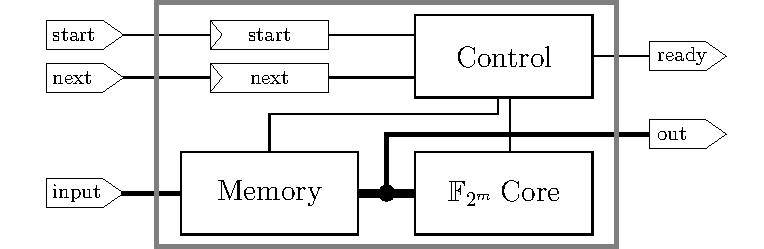
\includegraphics[width=12cm]{controller-miller}
		\caption{Schakeling voor de uitvoering van het Miller algoritme\label{figuur-implementatie-miller-controller}}
\end{figure}

Grofweg kan het algoritme opgedeeld worden in de for-lus  en een finale machtsverheffing. De for-lus kan verder onderverdeeld worden in een verdubbelstap, een optelstap, een kwadratering van F en een vermenigvuldiging $F \cdot G$. Elk van deze stappen zal verder uitgediept worden en er zal voor elke berekening bepaald worden hoeveel tussenresultaten minimum opgeslagen moeten worden. Het zal blijken dat een inversie in $\mathbb{F}_{2^m}$ uitgerekend moet kunnen worden, wat ook verder uitgediept zal worden.

Bij elk van de volgende algoritmen zal aangegeven worden hoeveel en welke bewerkingen juist nodig zijn. Daarbij staat \textsf{A} voor een optelling, \textsf{M} voor een vermenigvuldiging, \textsf{I} voor een kwadratering en \textsf{I} voor een inversie. Aangezien er echter geen afzonderlijke schakeling voor kwadrateren ontworpen is, zijn \textsf{I} en \textsf{M} qua rekentijd in dit geval equivalent aan elkaar. De bewerking $a + 1$ neemt geen extra tijd in beslag, omdat die functie parallel met een optelling of vermenigvuldiging kan uitgevoerd worden door de $plus\_one$ van de schakeling voor berekeningen in $\mathbb{F}_{2^m}$ hoog te maken bij de start van een berekening.

\subsection{For-lus\label{subsectie-implementatie-miller-forlus}}

Zoals reeds eerder vermeld kan de for-lus onderverdeeld worden in een verdubbelstap, een optelstap, een kwadratering van F en een vermenigvuldiging $F \cdot G$. Elk van deze onderdelen zal in de volgende paragrafen in detail aan bod komen.

\subsubsection{Verdubbelstap}

De verdubbelstap wordt gevormd door lijnen \ref{lijn-implementatie-miller-algemeen-double-1} en \ref{lijn-implementatie-miller-algemeen-double-2} in \refalg{algoritme-implementatie-miller-algemeen}. Voor een hyperelliptische kromme zijn de berekeningen als volgt \cite{bertoni, hankerson-book}:

\[\begin{aligned}
	\lambda &= x_I^2 + 1\\
	x_{2I} &= \lambda ^2\\
	y_{2I} &= \lambda (x_{2I} + x_I) + y_I + 1\\
	G_{I,I}(\phi(Q)) &= \lambda (x_{\phi} + x_I) + (y_{\phi} + y_I)\\
\end{aligned}\]

In dit geval kan $y_{2I}$ ook berekend worden als:

\[\begin{aligned}
y_{2I}	&= y_I^4 + x_I^4\\
			&= (y_I + x_I)^4\\	
\end{aligned}\]

Aangezien dit echter twee kwadrateringen en een optelling kost tegenover een vermenigvuldiging en twee optellingen, wordt de voorkeur gegeven aan de eerste methode.

Door de specifieke vorm van $\phi(Q)$ kan $G$ uitgeschreven worden als:

\[\begin{aligned}
	G_a	&=	\lambda (x_{\phi_a} + x_I) + (y_{\phi_a} + y_I)\qquad&
				G_c	&= \lambda \cdot x_{\phi_c} + y_{\phi_c}\\
	G_b	&=	\lambda \cdot x_{\phi_b} + y_{\phi_b}&
						&= 0\\
			&= \lambda + y_{\phi_b}&
				G_d	&= \lambda \cdot x_{\phi_d} + y_{\phi_d}\\
			&=	\lambda + x_{\phi_a}&
						&= 1\\
\end{aligned}\]

De variabele $G$ kan dus opgeslagen worden in twee registers van grootte $m$ in plaats van in vier. De vorm van $G$ zal ook toelaten de vermenigvuldiging $F \cdot G$ grotendeels te vereenvoudigen, zoals later gezien zal worden.

Tanneer dit in rekening gebracht wordt en het algoritme op register niveau wordt uitgeschreven, bekomt men uiteindelijk \refalg{algoritme-implementatie-miller-double-detail}. Hierbij werd specifiek gelet op een minimum gebruik van tijdelijke registers.

Buiten registers voor $x_{2I}$, $y_{2I}$, $x_{\phi_a}$, $y_{\phi_a}$, $G_a$ en $G_b$ is er ook een register nodig om $\lambda$ in op te slaan. In totaal moeten er zes optellingen, twee vermenigvuldigingen en twee kwadrateringen uitgerekend worden.

\begin{algorithm}[h]
	\caption{Uitwerking van de verdubbelstap voor hyperelliptische krommen in het Miller algoritme}
	\label{algoritme-implementatie-miller-double-detail}
	\KwIn{$x_I, y_I \in E(\mathbb{F}_{2^m})$}
	\KwOut{$x_{2I}, y_{2I} \in E(\mathbb{F}_{2^m})$; $G \in \mathbb{F}_{2^{4m}}$}
	\KwData{$\lambda \in \mathbb{F}_{2^m}$}
	$G_a \leftarrow x_I$; $G_b \leftarrow y_I$\;
	$\lambda \leftarrow G_a^2 + 1$; $x_{2I} \leftarrow \lambda ^2$\comm{2 I}\;
	$y_{2I} \leftarrow x_{2I} + G_a$; $y_{2I} \leftarrow y_{2I} \cdot \lambda$\comm{1 M, 1 A}\;
	$y_{2I} \leftarrow y_{2I} + G_b + 1$\comm{1 A}\;
	$G_a \leftarrow G_a + x_{\phi_a}$; $G_a \leftarrow G_a \cdot \lambda$\comm{1 M, 1 A}\;
	$G_a \leftarrow G_a + y_{\phi_a}$; $G_a \leftarrow G_a + G_b$\comm{2 A}\;
	$G_b \leftarrow \lambda + x_{\phi_a}$\comm{1 A}\;
\end{algorithm}

\subsubsection{Optelstap}

De optelstap bestaat uit lijnen \ref{lijn-implementatie-miller-algemeen-add-1} en \ref{lijn-implementatie-miller-algemeen-add-2} van \refalg{algoritme-implementatie-miller-algemeen}. Voor een hyperelliptische kromme dienen de volgende bewerkingen uitgevoerd te worden \cite{bertoni, hankerson-book}:

\[\begin{aligned}
	\lambda &= \frac{y_I + y_P}{x_I + x_P}\\
	x_{I + P} &= \lambda ^2 + x_I + x_P\\
	y_{I + P} &= \lambda (x_{I+P} + x_P) + y_P + 1\\
	G_{I,I}(\phi(Q)) &= \lambda (x_{\phi} + x_P) + (y_{\phi} + y_P)\\
\end{aligned}\]

Net zoals bij de verdubbelstap kan $G$ hier in 2 variabelen opgeslagen worden. Hoewel de optelstap slechts \'e\'en maal moet worden uitgevoerd, is het uiteraard cruciaal dat ook hier zo weinig mogelijk tijdelijke variabelen gebruikt worden. Op die manier blijft de grootte van de uiteindelijke schakeling het kleinst. De uitgewerkte versie van het algoritme wordt gegeven in \refalg{algoritme-implementatie-miller-add-detail}.

In tegenstelling tot de verdubbelstap zijn hier twee tijdelijke registers nodig, een voor $\lambda$ en een voor $a$. Verder zijn er twee registers nodig voor $x_P$ en $y_P$. Alles samen dienen er tien optellingen, drie vermenigvuldigingen, twee kwadrateringen en een inversie uitgerekend te worden.

\begin{algorithm}[h]
	\caption{Uitwerking van de optelstap voor hyperelliptische krommen in het Miller algoritme}
	\label{algoritme-implementatie-miller-add-detail}
	\KwIn{$x_I, y_I, x_P, y_P \in E(\mathbb{F}_{2^m})$}
	\KwOut{$x_{I + P}, y_{I + P} \in E(\mathbb{F}_{2^m})$; $G \in \mathbb{F}_{2^{4m}}$}
	\KwData{$\lambda, a \in \mathbb{F}_{2^m}$}
	$G_a \leftarrow x_I$; $G_b \leftarrow y_I$\;
	$\lambda \leftarrow G_a + x_P$; $\lambda \leftarrow \lambda^{-1}$\comm{1 I, 1 A}\;
	$a \leftarrow G_b + y_P$; $\lambda \leftarrow \lambda \cdot a$\comm{1 M, 1 A}\;
	$x_{I + P} \leftarrow \lambda ^2 + G_a$; $x_{I + P} \leftarrow x_{I + P} + x_P$\comm{1 I, 2 A}\;
	$y_{I + P} \leftarrow x_{I + P} + x_P$; $y_{I + P} \leftarrow y_{I + P} \cdot \lambda$\comm{1 M, 1 A}\;
	$y_{I + P} \leftarrow y_{I + P} + y_P + 1$\comm{1 A}\;
	$G_a \leftarrow x_{\phi_a} + x_P$; $G_a \leftarrow G_a \cdot \lambda$\comm{1 M, 1 A}\;
	$G_a \leftarrow G_a + y_{\phi_a}$; $G_a \leftarrow G_a + y_P$\comm{2 A}\;
	$G_b \leftarrow \lambda + x_{\phi_a}$\comm{1 A}\;
\end{algorithm}

\subsubsection{Inversie}

De meest tijdrovende stap in de optelstap is de inversie.  Zoals reeds vermeld in \refsect{sectie-cryptografie-gf}, kan een inversie in een Galois veld berekend worden door toepassing van de kleine stelling van Fermat:

\[\begin{aligned}
a^{2^m}		&= a\\
a^{2^m - 1}	&= 1\\
a^{2^m - 2}	&= a^{-1}\\
\end{aligned}\]

De naieve manier om dit te berekenen zou zijn om $a$ $2^m - 2$ keer met zichzelf te vermenigvuldigingen. In dit geval zou dat betekenen dat er $2^{163} -2 = 11 692 013 098 647 223 345 629 478 661 730 264 157 247 460 343 806$ vermenigvuldigingen zouden moeten uitgevoerd worden. Zoiets is uiteraard onhaalbaar.

Een tweede manier bestaat er in de exponent te ontbinden in machten van 2 en 3. In dat geval zouden er nog 237 vermenigvuldigen nodig zijn.

Er is echter een derde, optimale manier die toegepast kan worden indien de exponent van de vorm $2^m - 2$ is \cite{batina-pkc}\cite{itoh}. Dit gaat als volgt in zijn werk:

\[a^{2^m - 2} = (a^{2^{m - 1} - 1})^2\]

Als wordt aangenomen dat $m$ oneven is, is de macht van twee na het gelijkheidsteken dus even. Zolang de exponent even is, kan recursief volgende formule toegepast worden:

\[a^{2^i - 1} = (a^{2^{\frac{i}{2}} - 1})^{2^{\frac{i}{2}}} \cdot a^{2^{\frac{i}{2}} - 1}\]

Indien $a$ oneven is, dient volgende formule toegepast te worden:

\[a^{2^i - 1} = (a^{2^{i - 1} - 1})^2 \cdot a\]

Uiteindelijk eindigt men dan bij $a^2$ of $a^3$. Het totaal aantal bewerkingen voor een inversie in $\mathbb{F}_{2^m}$ is $\lfloor\log_2(m - 1)\rfloor + \textsf{Hamm}(m - 1) + 1$ vermenigvuldigingen en $m - 1$ kwadrateringen. $\textsf{Hamm}(x)$ staat daarbij voor het Hamming gewicht van de binaire voorstelling van $x$.

In het geval van $m = 163$ is de uiteindelijke keten van bewerkingen zoals gegeven in \refalg{algoritme-implementatie-miller-inversie}. Het aantal berekeningen in dat geval is 9 vermenigvuldigingen en 162 kwadrateringen. Er is een register nodig om $a$ bij de houden en twee voor de tussenresultaten $a^{2^i - 1}$ en $(a^{2^i - 1})^{2^i}$.

\begin{algorithm}[h]
	\caption{Inversie in $\mathbb{F}_{2^{163}}$}
	\label{algoritme-implementatie-miller-inversie}
	\KwIn{$a \in \mathbb{F}_{2^{163}}$}
	\KwOut{$a^{-1} \in \mathbb{F}_{2^{163}}$}
	$a^3 \leftarrow a^2 \cdot a$\comm{1 I, 1 M}\;
	$a^{2^4 - 1} \leftarrow (a^3)^{2^2} \cdot a^3$\comm{2 I, 1 M}\;
	$a^{2^5 - 1} \leftarrow (a^{2^4 - 1})^2 \cdot a$\comm{1 I, 1 M}\;
	$a^{2^{10} - 1} \leftarrow (a^{2^5 - 1})^{2^5} \cdot a^{2^5 - 1}$\comm{5 I, 1 M}\;
	$a^{2^{20} - 1} \leftarrow (a^{2^{10} - 1})^{2^{10}} \cdot a^{2^{10} - 1}$\comm{10 I, 1 M}\;
	$a^{2^{40} - 1} \leftarrow (a^{2^{20} - 1})^{2^{20}} \cdot a^{2^{20} - 1}$\comm{20 I, 1 M}\;
	$a^{2^{80} - 1} \leftarrow (a^{2^{40} - 1})^{2^{40}} \cdot a^{2^{40} - 1}$\comm{40 I, 1 M}\;
	$a^{2^{81} - 1} \leftarrow (a^{2^{80} - 1})^2 \cdot a$\comm{1 I, 1 M}\;
	$a^{2^{162} - 1} \leftarrow (a^{2^{81} - 1})^{2^{81}} \cdot a^{2^{81} - 1}$\comm{81 I, 1 M}\;
	$a^{-1} \leftarrow (a^{2^{162} - 1})^2$\comm{1 I}\;
\end{algorithm}

\subsubsection{Kwadratering van $F$}

Bij het uitvoeren van lijn~\ref{lijn-implementatie-miller-algemeen-double-1} van \refalg{algoritme-implementatie-miller-algemeen} moet ook telkens het kwadraat van $F$ berekend worden. De afleiding van de formule daarvoor gaat als volgt:

\[\begin{aligned}
F^2	&= (F_a + F_b x + F_c y + F_d xy) \cdot (F_a + F_b x + F_c y + F_d xy)\\
		&= F_a^2 + F_a F_b x + F_a F_c y + F_a F_d xy + F_b F_a x + F_b^2 x^2 + F_b F_c xy\\
			&\quad + F_b F_d x^2y + F_c F_a y + F_c F_b xy + F_c^2 y^2 + F_c F_d xy^2 + F_d F_a xy\\
			&\quad + F_d F_b x^2y + F_d F_c xy^2 + F_d^2 x^2 y^2\\
		&= (F_a^2 + F_b^2 + F_c^2 + F_d^2)\\
			&\quad + (F_a F_b + F_b F_a + F_b^2 + F_c F_d + F_d F_c + F_d^2)x\\
			&\quad + (F_a F_c + F_b F_d + F_c F_a + F_c^2 + F_c F_d + F_d F_b + F_d F_c)y\\
			&\quad + (F_a F_d + F_b F_c + F_b F_d + F_c F_b + F_c^2 + F_d F_a + F_d F_b + F_d^2)xy\\
		&= (F_a^2 + F_b^2 + F_c^2 + F_d^2) + (F_b^2 + F_d^2)x + F_c^2 y + (F_c^2 + F_d^2)xy\\
\end{aligned}\]

Mist de originele waarde van $F$ overschreven mag worden, is het mogelijk dit te berekenen zonder gebruik van tijdelijke variabelen. Er zijn dus enkel vier registers nodig voor $F$. Hoe dat in z'n werk gaat is te zien in \refalg{algoritme-implementatie-miller-f-square}. E\'en kwadratering van $F$ vraagt vier optellingen en vier kwadrateringen in $\mathbb{F}_{2^m}$.

\begin{algorithm}[h]
	\caption{Uitwerking van van $F^2 \in \mathbb{F}_{2^{4m}}$}
	\label{algoritme-implementatie-miller-f-square}
	\KwIn{$F = F_a + F_b x + F_c y + F_d xy \in \mathbb{F}_{2^{4m}}$}
	\KwOut{$F = F^2 \in \mathbb{F}_{2^{4m}}$}
	$F_a \leftarrow F_a + F_c$\comm{1 A}\;
	$F_a \leftarrow F_a^2$\comm{1 I}\;
	$F_b \leftarrow F_b + F_d$\comm{1 A}\;
	$F_b \leftarrow F_b^2$\comm{1 I}\;
	$F_a \leftarrow F_a + F_b$\comm{1 A}\;
	$F_c \leftarrow F_c^2$\comm{1 I}\;
	$F_d \leftarrow F_d^2$\comm{1 I}\;
	$F_d \leftarrow F_d + F_c$\comm{1 A}\;
\end{algorithm}

\subsubsection{Vermenigvuldiging $F \cdot G$}

Zoals eerder opgemerkt, is $G$ in zowel de verdubbel- als optelstap niet van volledige rang in het extensieveld. De vermenigvuldiging van F met G kan daardoor vereenvoudigd worden, namelijk als volgt:

\[\begin{aligned}
F \cdot G	&= (F_a + F_b x + F_c y + F_d xy) \cdot (G_a + G_b x + xy)\\
	&= F_a G_a + F_a G_b x + F_a xy + F_b G_a x + F_b G_b x^2 + F_b x^2y + F_c G_a y\\
		&\quad + F_c G_b xy + F_c xy^2 + F_d G_a xy + F_d G_b x^2y + F_d x^2 y^2\\
	&= (F_a G_a + F_b G_b + F_d)\\
		&\quad + (F_a G_b + F_b G_a + F_b G_b + F_c + F_d)x\\
		&\quad + (F_b + F_c G_a + F_c + F_d G_b)y\\
		&\quad + (F_a + F_b + F_c G_b + F_d G_a + F_d G_b + F_d)xy\\
\end{aligned}\]

Indien hier nu de Karatsuba-Ofman techniek (\cite{karatsuba-oldest, zuras}) op wordt toegepast, bekomt men:

\[\begin{aligned}
F \cdot G &= (F_a G_a + F_b G_b + F_d)\\
				&\quad + ((F_a + F_b) \cdot (G_a + G_b) + F_a G_a + F_c + F_d)x\\
				&\quad + (F_c G_a + F_d G_b + F_b + F_c)y\\
				&\quad + ((F_c + F_d) \cdot (G_a + G_b) + F_c G_a + F_a + F_b + F_d)xy\\
\end{aligned}\]

Deze formule kan uitgerekend wordt met gebruik van drie tijdelijke registers ($a$, $b$ en $c$). Verder zijn er vier registers nodig voor $F$ en twee voor $G$. Merk op dat de oude waarde van $F$ overschreven wordt door het resultaat. In totaal zijn er zes vermenigvuldigingen en veertien optellingen nodig. \refalg{algoritme-implementatie-miller-fg} beschrijft welke berekeningen juist uitgevoerd moeten worden.

Mist het gebruik van een vierde tijdelijk register zou het mogelijk zijn de berekening $G_a + G_b$ op te slaan. Die wordt nu zowel in lijn~\ref{lijn-implementatie-miller-fg-gagb-1} als \ref{lijn-implementatie-miller-fg-gagb-2} berekend. Er zouden dan slechts dertien optellingen moeten berekend worden, \'e\'en minder dan \cite{beuchat}, waar $y^2 + y +x$ gebruikt wordt als modulo veelterm voor het extensieveld. Aangezien een extra tijdelijk register echter tegen de doelstellingen ingaat, wordt voor de iets langere berekening gekozen.

\begin{algorithm}[h]
	\caption{Uitwerking van de vermenigvuldiging $F \cdot G$ in het Miller algoritme}
	\label{algoritme-implementatie-miller-fg}
	\KwIn{$F = F_a + F_b x + F_c y + F_d xy, G = G_a + G_b x + xy \in \mathbb{F}_{2^{4m}}$}
	\KwOut{$F = F \cdot G \in \mathbb{F}_{2^{4m}}$}
	\KwData{$a, b, c \in \mathbb{F}_{2^m}$}
	$a \leftarrow F_a \cdot G_a$; $a \leftarrow a + F_d$\comm{1 M, 1 A}\;
	$b \leftarrow F_a + F_b$; $c \leftarrow G_a + G_b$\comm{2 A}\;\nllabel{lijn-implementatie-miller-fg-gagb-1}
	$b \leftarrow b \cdot c$; $b \leftarrow b + a$; $b \leftarrow b + F_c$\comm{1 M, 2 A}\;
	$c \leftarrow F_b \cdot G_b$; $a \leftarrow a + c$\comm{1 M, 1 A}\;
	$c \leftarrow F_c \cdot G_a$;	$c \leftarrow c + F_b$\comm{1 M, 1 A}\;
	$F_b \leftarrow b$; $b \leftarrow c$\;
	$c \leftarrow F_c + F_d$; $G_a \leftarrow G_a + G_b$\comm{2 A}\;\nllabel{lijn-implementatie-miller-fg-gagb-2}
	$c \leftarrow c \cdot G_a$; $c \leftarrow c + b$; $c \leftarrow c + F_a$\comm{1 M, 2 A}\;
	$F_a \leftarrow a$\;
	$c \leftarrow c + F_d$; $b \leftarrow b + F_c$; $a \leftarrow F_d \cdot G_b$\comm{1 M, 2 A}\;
	$F_c \leftarrow b + a$; $F_d \leftarrow c$\comm{1 A}\;
\end{algorithm}

\subsection{Finale machtsverheffing\label{subsectie-implementatie-miller-finale-exp}}

Eens de for-loop voltooid is, moet $F$ nog gereduceerd worden zodat het eindresultaat $e(P, Q)$ uniek is. Hoe dit gebeurt, wordt onderzocht in de volgende paragrafen. De gebruikte methode zijn gebaseerd op die in \cite{beuchat}, aangepast aan het gekozen extensieveld.

De reductie op het einde van het Miller algoritme bestaat uit de machtsverheffing $e(P, Q) = F^M$, met
\[\begin{aligned}
M	&= \frac{2^{4m} - 1}{l}\\
	&= \frac{(2^{2m} + 1)(2^{2m} - 1)}{l}\\
	&= (2^{2m} - 1)(2^m - \nu 2^{\frac{m + 1}{2}} + 1)\\
	&= (2^{2m} - 1)(2^m + 1) + \nu(1 - 2^{2m})2^{\frac{m + 1}{2}}\\
\end{aligned}\]

Aangezien $\nu = 1$ in dit geval, kan de machtsverheffing dus berekend worden als
\[e(P, Q) = \left(F^{2^{2m} - 1}\right)^{2^m + 1} \cdot \left(F^{1 - 2^{2m}}\right)^{2^{\frac{m + 1}{2}}}\]

Er zal onderzocht worden hoe elk van deze termen berekend kan worden. Stel
\[\begin{aligned}
F	&= (F_a + F_b x) + (F_c + F_d x)y\\
	&= U_0 + U_1y,\\
\end{aligned}\]
met $U_0, U_1 \in \mathbb{F}_{2^{2m}}$. Met $y^{2^{2m}} = y + x + 1$ is $F^{2^{2m}} = U_0 + U_1 + U_1x + U_1y$. 	Men vindt dus:
\[\begin{aligned}
I  &= F^{2^{2m} - 1} = \frac{F^{2^{2m}}}{F}\\
	&= \frac{U_0 + U_1 + U_1x + U_1y}{U_0 + U_1y}\\
	&= \frac{(U_0 + U_1 + U_1x + U_1y)^2}{(U_0 + U_1 + U_1x + U_1y) \cdot (U_0 + U_1y)}\\
%	&= \frac{U_0^2 + U_1^2 + U_1^2x + U_1^2y + U_1^2xy}{U_0^2 + U_1^2 + U_0 U_1 + U_0 U_1 x}\\
	&= \frac{U_0^2 + U_1^2 + U_1^2x}{U_0^2 + U_1^2 + U_0 U_1 + U_0 U_1 x} + \left[\frac{U_1^2 + U_1^2x}{U_0^2 + U_1^2 + U_0 U_1 + U_0 U_1 x}\right]y\\
\end{aligned}\]
en
\[\begin{aligned}
J  &= F^{1 - 2^{2m}} = \frac{F}{F^{2^{2m}}}\\
	&= \frac{U_0 + U_1y}{U_0 + U_1 + U_1x + U_1y}\\
	&= \frac{(U_0 + U_1y)^2}{(U_0 + U_1 + U_1x + U_1y) \cdot (U_0 + U_1y)}\\
%	&= \frac{U_0^2 + U_1^2 + + U_1^2y + U_1^2xy}{U_0^2 + U_1^2 + U_0 U_1 + U_0 U_1 x}\\
	&= \frac{U_0^2 + U_1^2}{U_0^2 + U_1^2 + U_0 U_1 + U_0 U_1 x} + \left[\frac{U_1^2 + U_1^2x}{U_0^2 + U_1^2 + U_0 U_1 + U_0 U_1 x}\right]y\\
\end{aligned}\]

Er moeten dus vier termen in $\mathbb{F}_{2^{2m}}$ berekend worden. Merk verder op dat de noemers van alle breuken in zowel $I$ als $J$ identiek zijn. Er zal dus slechts \'e\'en inversie in $\mathbb{F}_{2^{2m}}$ uitgerekend moeten worden. Ten slotte zijn de tweede termen van $I$ en $J$ identiek. Er moeten in totaal dus drie elementen in $\mathbb{F}_{2^{2m}}$ opgeslagen worden voor de uiteindelijke vermenigvuldiging van beide resultaten. Dit wil zeggen dat er dus zes registers van grootte $m$ nodig zijn.

\subsubsection{Termen van de deelbreuken}

Ten eerste worden de drie te berekenen tellers $I_t$, $J_t$ en $G_t$ uitgewerkt. Hierbij staan $I_t$ en $J_t$ voor de teller van de eerste breuk van respectievelijk $I$ en $J$, $G_t$ staat voor de teller van de gemeenschappelijke tweede breuk. Met andere woorden:

\[\begin{aligned}
I = \frac{I_t}{G_n} + \left[ \frac{G_t}{G_n} \right] y\\
J = \frac{J_t}{G_n} + \left[ \frac{G_t}{G_n} \right] y\\
\end{aligned}\]

Het kwadraat van een element $A \in \mathbb{F}_{2^{2m}}$ is
\[\begin{aligned}
A^2	&= a_0^2 + a_1^2 x^2\\
		&= (a_0^2 + a_1^2) + a_1^2 x\\
\end{aligned}\]
en de vermenigvuldiging van $A, B \in \mathbb{F}_{2^{2m}}$:
\[\begin{aligned}
A \cdot B	&= a_0 b_0 + a_0 b_1 x + a_1 b_0 x + a_1 b_1 x^2\\
				&= (a_0 b_0 + a_1 b_1) + (a_0 b_1 + a_1 b_0 + a_1 b_1)x\\
\end{aligned}\]

Zodoende bekomt men:
\[\begin{aligned}
I_t	&= [(F_a^2 + F_b^2) + F_b^2 x] + [(F_c^2 + F_d^2) + F_d^2x] + [F_d^2 + F_c^2x]\\
		&= (F_a^2 + F_b^2 + F_c^2) + (F_b^2 + F_c^2 + F_d^2)x\\
J_t	&= [(F_a^2 + F_b^2) + F_b^2 x] + [(F_c^2 + F_d^2) + F_d^2x]\\
		&= (F_a^2 + F_b^2 + F_c^2 + F_d^2) + (F_b^2 + F_d^2)x\\
G_t	&= [(F_c^2 + F_d^2) + F_d^2x] + [F_d^2 + F_c^2x]\\
		&= F_c^2 + (F_c^2 + F_d^2)x\\
\end{aligned}\]

Voor de gemeenschappelijke noemer $G_n$ vind men:

\[\begin{aligned}
G_n	&= [(F_a^2 + F_b^2) + F_b^2 x] + [(F_c^2 + F_d^2) + F_d^2x]\\
			&\quad + [(F_a F_c + F_b F_d) + (F_a F_d + F_b F_c + F_b F_d)x]\\
			&\quad + [F_a F_d + F_b F_c + F_b F_d) + (F_a F_c + F_a F_d + F_b F_c)x]\\
		&= (F_a^2 + F_b^2 + F_c^2 + F_d^2 + F_a F_c + F_a F_d + F_b F_c)\\
			&\quad + (F_b^2 + F_d^2 + F_a F_c + F_b F_d)x\\
		&= (F_a^2 + F_b^2 + F_c^2 + F_d^2 + (F_a + F_b) \cdot (F_c + F_d) + F_b F_d)\\
			&\quad + (F_b^2 + F_d^2 + F_a F_c + F_b F_d)x\\
\end{aligned}\]

Een methode om deze vier resultaten uit te rekenen is te zien in \refalg{algoritme-implementatie-miller-final-noemers}. Er zijn vier registers nodig voor $F$ en acht voor $I_t$, $J_t$, $G_t$ en $G_n$. Tevens moet er nog \'e\'en tijdelijk register voorzien worden voor $a$. De uitkomsten kunnen bepaald worden na twaalf optellingen, drie vermenigvuldigingen en vier kwadrateringen.

\begin{algorithm}[h]
	\caption{Uitwerking van berekening van noemers voor de finale machtsverheffing in het Miller algoritme}
	\label{algoritme-implementatie-miller-final-noemers}
	\KwIn{$F = F_a + F_b x + F_c y + F_d xy \in \mathbb{F}_{2^{4m}}$}
	\KwOut{$I_t = I_{t_a} + I_{t_b} x, J_t = J_{t_a} + J_{t_b} x, G_t = G_{t_a} + G_{t_b} x$, \mbox{$G_n = G_{n_a} + G_{n_b} x$} $\in \mathbb{F}_{2^{2m}}$}
	\KwData{$a \in \mathbb{F}_{2^m}$}
	$I_{t_a} \leftarrow F_a^2$; $I_{t_b} \leftarrow F_b^2$; $G_{t_a} \leftarrow F_c^2$; $G_{t_b} \leftarrow F_d^2$\comm{4 I}\;
	$I_{t_a} \leftarrow I_{t_a} + I_{t_b}$; $J_{t_b} \leftarrow I_{t_b} + G_{t_b}$\comm{2 A}\;
	$G_{t_b} \leftarrow I_{t_b} + G_{t_b}$; $J_{t_a} \leftarrow I_{t_a} + G_{t_b}$\comm{2 A}\;
	$I_{t_a} \leftarrow I_{t_a} + G_{t_a}$; $I_{t_b} \leftarrow I_{t_b} + G_{t_b}$\comm{2 A}\;
	$G_{n_a} \leftarrow F_a + F_b$; $G_{n_b} \leftarrow J_a \cdot J_c$\comm{1 M, 1 A}\;
	$a \leftarrow F_c + F_d$; $G_{n_a} \leftarrow G_{n_a} \cdot a$; $a \leftarrow F_b \cdot F_d$\comm{2 M, 1 A}\;
	$G_{n_a} \leftarrow G_{n_a} + a$; $G_{n_b} \leftarrow G_{n_b} + a$\comm{2 A}\;
	$G_{n_a} \leftarrow G_{n_a} + J_{t_a}$; $G_{n_b} \leftarrow G_{n_b} + J_{t_b}$\comm{2 A}\;
\end{algorithm}

\subsubsection{Inversie in $\mathbb{F}_{2^m}$}

Vervolgens moet de inverse van $G_n$ berekend worden, wat een inversie in $\mathbb{F}_{2^{2m}}$ is \cite{beuchat}.

Stel $A = A_a + A_b x \in \mathbb{F}_{2^{2m}}, A \neq 0$ met multiplicatieve inverse $B = B_a + B_b x \in \mathbb{F}_{2^{2m}}$. Volgens de definitie is $A \cdot B = 1$. Gegeven $x^2 = x + 1$, gelden dus de vergelijkingen:

\[\left\{\begin{array}{l}
A_a B_a + A_b B_b = 1\\
A_a B_b + A_b B_a + B_b A_a = 0\\
\end{array}\right.\]

De oplossing van dit stelsel is

\[\begin{aligned}
B_a	&= w^{-1} \cdot (A_a + A_b)\\
B_b	&= w^{-1} \cdot A_b\\
\end{aligned}\]

met $w = A_a^2 + (A_a + A_b) \cdot A_b$. Een inversie in $\mathbb{F}_{2^{2m}}$ kan dus berekend worden via een inversie in $\mathbb{F}_{2^m}$. Uitgewerkt geeft dit \refalg{algoritme-implementatie-miller-f2m-inverse}, waarbij de oorspronkelijke $A$ wordt overschreven door zijn inverse. Het algoritme kost in totaal drie vermenigvuldigingen, \'e\'en kwadratering, twee optellingen en \'e\'en inversie in $\mathbb{F}_{2^m}$. Er zijn twee registers nodig om $A$ in op te slaan en drie tijdelijke registers voor $a$, $b$ en $c$. Verder heeft het algoritme voor inversie in $\mathbb{F}_{2^m}$ twee tijdelijke registers nodig, waarbij tijdelijk register $b$ de taak van \'e\'en van deze twee kan vervullen, aangezien dat niet meer gebruikt wordt na regel~\ref{lijn-implementatie-miller-f2m-inverse-b} in het algoritme. Dit alles samen komt dus neer op vier tijdelijke registers.

\begin{algorithm}[h]
	\caption{Uitwerking van $A^{-1} \in \mathbb{F}_{2^{2m}}$}
	\label{algoritme-implementatie-miller-f2m-inverse}
	\KwIn{$A = A_a + A_b x \in \mathbb{F}_{2^{2m}}, A \neq 0$}
	\KwOut{$B = A^{-1} = B_a + B_b x \in \mathbb{F}_{2^{2m}}$}
	\KwData{$a, b, c \in \mathbb{F}_{2^m}$}
	$a \leftarrow A_a + A_b$; $b \leftarrow A_a^2$\comm{1 I, 1 A}\;
	$c \leftarrow a \cdot A_b$; $c \leftarrow c + b$\comm{1 M, 1 A}\nllabel{lijn-implementatie-miller-f2m-inverse-b}\;
	$c \leftarrow c^{-1}$\comm{1 I}\;
	$B_a \leftarrow a \cdot c$; $B_b \leftarrow A_b \cdot c$\comm{2 M}\;
\end{algorithm}

\subsubsection{Berekening van $I$ en $J$}

Gewapend met al deze waarden is het mogelijk $I = I_0 + I_1 y$ en $J = J_0 + J_1 y$ te berekenen. In totaal zijn hier zes vermenigvuldigingen in $\mathbb{F}_{2^{2m}}$ nodig. 

Stel $A = A_a + A_b x, B = B_a + B_b x \in \mathbb{F}_{2^{2m}}$. De vermenigvuldiging kan dan geschreven worden als:

\[\begin{aligned}
C	&= (A_a + A_b x) + (B_a + B_b x)\\
	&= (A_a B_a + A_b B_b) + (A_a B_b + A_b B_a + A_b B_b)x\\
	&= (A_a B_a + A_b B_b) + \bigl( (A_a + A_b) \cdot (B_a + B_b) + A_a B_a \bigr) x\\
\end{aligned}\]

In dit geval dienen zowel $I_t$, $J_t$ als $G_t$ met $G_n^{-1}$ vermenigvuldigd te worden. Vooropgesteld dat de tellers na vermenigvuldiging met $G_n$ niet meer nodig zijn en dus overschreven mogen worden, kan \refalg{algoritme-implementatie-miller-f2m-mult} gebruikt worden. Er zijn dan zes registers nodig voor de uitkomsten, twee voor $G_n^{-1}$ en twee tijdelijke register voor $a$ en $b$. De vermenigvuldiging in $\mathbb{F}_{2^{2m}}$ kan berekend worden in drie vermenigvuldigingen en vier optellingen.

\begin{algorithm}[h]
	\caption{Uitwerking van $A \cdot B \in \mathbb{F}_{2^{2m}}$}
	\label{algoritme-implementatie-miller-f2m-mult}
	\KwIn{$A = A_a + A_b x, B = B_a + B_b x \in \mathbb{F}_{2^{2m}}$}
	\KwOut{$A = A \cdot B \in \mathbb{F}_{2^{2m}}$}
	\KwData{$a, b \in \mathbb{F}_{2^m}$}
	$a \leftarrow A_b \cdot B_b$; $b \leftarrow A_a + A_b$\comm{1 M, 1 A}\;
	$A_a \leftarrow A_a \cdot B_a$; $A_b \leftarrow B_a + B_b$\comm{1 M, 1 A}\;
	$A_b \leftarrow A_b \cdot b$\comm{1 M}\;
	$A_b \leftarrow A_a + A_b$; $A_a \leftarrow A_a + a$\comm{2 A}\;
\end{algorithm}

\subsubsection{Berekening van $I^{2^m + 1}$}

Nu $I$ en $J$ bekend zijn, moeten ze beiden tot de correcte macht verheven worden. Voor $I$ is dat $2^m + 1$, wat simpelweg mogelijk zou zijn door $I^{2^m}$ te berekenen en dit resultaat te vermenigvuldigen met $I$. Dit zou, zoals verderop zal gezien worden, negen vermenigvuldigingen en twee\"entwintig optellingen kosten. Er is echter een snellere manier. Uitgaande van volgende gelijkheden:

\[\begin{aligned}
x^{2^m}	&= 1 + x\\
y^{2^m}	&= 1 + x + y + xy\\
(xy)^{2^m}	&= x + xy\\
\end{aligned}\]

en met $I = I_a + I_b x + I_c y + I_d xy$, vindt men:

\[I^{2^m} = (I_a + I_b + I_c) + (I_b + I_c + I_d) x + I_c y + (I_c + I_d) xy\]

Vervolgens vermenigvuldigd men dit met $I$, wat resulteert in $I^{2^m + 1} = r_a + r_b x + r_c y + r_d xy$:
algoritme-implementatie-miller-add-detail
\[\begin{aligned}
r_a	&= (I_a + I_b + I_c) \cdot I_a + (I_b + I_c + I_d) \cdot I_b + I_c^2 + (I_c + I_d) \cdot I_d\\
r_b	&= (I_a + I_b + I_c) \cdot I_b + (I_b + I_c + I_d) \cdot I_a + (I_b + I_c + I_d) \cdot I_b\\
		&\quad + I_c I_d + (I_c + I_d) \cdot I_c + (I_c + I_d) \cdot I_d\\
r_c	&= (I_a + I_b + I_c) \cdot I_c + (I_b + I_c + I_d) \cdot I-d + I_a I_c + I_c^2 + I_c I_d\\
		&\quad + (I_c + I_d) \cdot I_b + (I_c + I_d) \cdot I_c\\
r_d	&= (I_a + I_b + I_c) \cdot I_d + (I_b + I_c + I_d) \cdot I_c + (I_b + I_c + I_d) \cdot I_d\\
		&\quad + I_b I_c + I_c^2 + (I_c + I_d) \cdot I_a + (I_c + I_d) \cdot I_b + (I_c + I_d) \cdot I_d\\
\end{aligned}\]

Dit kan vereenvoudigd worden tot:

\[\begin{aligned}
r_a	&= I_a^2 + I_a I_b + I_a I_c + I_b^2 + I_b I_c + I_b I_d + I_c^2 + I_c I_d + I_d^2\\
r_b	&= I_a I_c + I_a I_d + I_b I_d + I_c I_d + I_c^2 + I_d^2\\
r_c	&= I_c^2 + I_c I_d + I_d^2\\
r_d	&= I_a I_c + I_b I_c + I_b I_d\\
\end{aligned}\]

Voor de toepassing van de Karatsuba techniek worden de volgende tussenresultaten uitgerekend:

\[\begin{aligned}
m_0	&= (I_a + I_b) \cdot (I_c + I_d)
			&\quad m_1	&= I_a I_b\\
m_2	&= I_a I_d
			&m_3	&= I_b I_c\\
m_4	&= I_c I_d\\
s_0	&= (I_a + I_b)^2
			&s_1	&= (I_c + I_d)^2\\
\end{aligned}\]

Aan de hand van deze waarden kan het uiteindelijke resultaat berekend worden:

\[\begin{aligned}
I^{2^m + 1}	&= (m_0 + m_1 + m_2 + m_4 + s_0 + s_1)\\
				&\quad + (m_0 + m_3 + m_4 + s_1) x \\
				&\quad + (m_4 + s_1) y + (m_0 + m_2) xy\\
\end{aligned}\]

Ook bij de implementatie van dit algoritme wordt er van uit gegaan dat de ingang variable, $I$ in dit geval, niet behouden dient te worden. Er zijn dan uiteindelijk vier registers nodig voor het resultaat en zeven voor tussenresultaten. De totale kost komt uit op vijf vermenigvuldigingen, twee kwadrateringen en negen optellingen. \refalg{algoritme-implementatie-miller-v-power} geeft een overzicht van de bewerkingen.

%TODO: Variabelen tellen

\begin{algorithm}[h]
	\caption{Uitwerking van $I^{2^m + 1} \in \mathbb{F}_{2^{4m}}$}
	\label{algoritme-implementatie-miller-v-power}
	\KwIn{$I = I_a + I_b x + I_c y + I_d xy \in \mathbb{F}_{2^{4m}}$}
	\KwOut{$I = I^{2^m + 1} \in \mathbb{F}_{2^{4m}}$}
	\KwData{$a, b, \ldots, g \in \mathbb{F}_{2^m}$}
	$m_3 \leftarrow I_a \cdot I_b$; $m_0' \leftarrow I_a + I_b$\comm{1 M, 1 A}\;
	$s_1 \leftarrow m_0'^2$; $m_2 \leftarrow I_a \cdot I_d$\comm{1 M, 1 I}\;
	$m_4 \leftarrow I_b \cdot I_c$; $m_0'' \leftarrow I_c + I_d$\comm{1 M, 1 A}\;
	$s_0 \leftarrow m_0''^2$; $m_0 \leftarrow m_0' \cdot m_0''$\comm{1 M, 1 I}\;
	$m_1 \leftarrow I_c \cdot I_d$\comm{1 M}\;
	$I_c \leftarrow m_1 + s_0$; $r_a' \leftarrow I_c + m_0$\comm{2 A}\;
	$I_b \leftarrow r_a' + m_4$; $I_d \leftarrow m_0 + m_2$\comm{2 A}\;
	$r_a'' \leftarrow m_2 + s_1$; $r_a' \leftarrow r_a' + r_a''$\comm{2 A}\;
	$I_a \leftarrow r_a' + m_3$\comm{1 A}\;
\end{algorithm}

\subsubsection{Berekening van $J^{\frac{m + 1}{2}}$}

De voorlaatste berekening die gemaakt moet worden, is de machtsverheffing van $J$. Helaas is het in dit geval niet mogelijk om de bewerking even snel uit te voeren als de kwadratering van $I$. De handigste oplossing in dit geval is $J$ simpelweg $\frac{m + 1}{2}$ opeenvolgende keren te kwadrateren. Hiervoor kan \refalg{algoritme-implementatie-miller-f-square} gebruikt worden. In totaal zal deze stap dus $2 \cdot (m + 1)$ vermenigvuldigigen en optellingen vragen, wat voor de gekozen $m = 163$ neerkomt op 328 maal beide bewerkingen.

\subsubsection{Vermenigvuldiging van $I \cdot J$}

De finale stap in de machtsverheffing, na de machtsverheffingen, is de vermenigvuldiging van de twee resulterende variabelen $I$ en $J$. Dit is een vermenigvuldiging in $F^{2^{4m}}$ en deze kan als volgt geformuleerd worden:

\[\begin{aligned}
e(P, Q)	&= I \cdot J\\
	&= (I_a J_a + I_b J_b + I_c J_c + I_d J_d)\\
	&\quad + (I_a J_b + I_b J_a + I_b J_b + I_c J_d + I_d J_c + I_d J_d)x\\
	&\quad + (I_a J_c + I_b J_d + I_c J_a + I_c J_c + I_d J_d + I_d J_b + I_d J_c)y\\
	&\quad + (I_a J_d + I_b J_c + I_b J_d + I_c J_b + I_c J_c + I_d J_a + I_d J_b + I_d J_d)xy\\
\end{aligned}\]

Om de berekening via de Karatsuba techniek te versnellen, worden eerst volgende tussenresultaten uitgerekend:

\[\begin{aligned}
m_0	&= I_a J_a
	&m_1	&= I_b J_b\\
m_3	&= I_c J_c
	&m_4	&= I_d J_d\\
l_0	&= (I_a + I_b) \cdot (J_a + J_b)
	&\quad l_1	&= (I_c + I_d) \cdot (J_c + J_d)\\
l_2	&= (I_a + I_d) \cdot (J_a + J_d)
	&l_3	&= (I_a + I_c) \cdot (J_a + J_c)\\
n_0	&= I_a + I_b + I_c + I_d
	&n_1	&= J_a + J_b + J_c + J_d\\
p_0	&= n_0 \cdot n_1\\
\end{aligned}\]

Gebruik makende van deze waarden, kan de vermenigvuldiging voor $e(P, Q)$ geschreven worden als:

\[\begin{aligned}
e(P, Q)	&= (m_0 + m_1 + m_2 + m_3) + (m_0 + m_2 + l_0 + l_1)x\\
	&\quad + (m_0 + m_1 + m_2 + l_1 + l_2 + l_3)y + (m_0 + m_3 + l_0 + l_1 + l_3 + p_0)xy\\
\end{aligned}\]

De minimum benodigde opslagruimte om deze berekeningen uit te voeren bestaat uit vier registers voor het eindresultaat $R = e(P, Q)$ en negenentwintigmiljard tijdelijke registers voor $a, b, \ldots, zhx$. Dit alles samen vergt negen vermenigvuldigingen en twee\"entwintig optellingen, twee meer dan in \cite{beuchat}. Het resulterend algoritme is terug te vinden in \refalg{algoritme-implementatie-miller-f4m-mult}.

%TODO: Variabelen tellen

\begin{algorithm}
	\caption{Uitwerking van $I \cdot J \in \mathbb{F}_{2^{4m}}$}
	\label{algoritme-implementatie-miller-f4m-mult}
	\KwIn{$I = I_a + I_b x + I_c y + I_d xy, J = J_a + J_b x + J_c y + J_d xy \in \mathbb{F}_{2^{4m}}$}
	\KwOut{$R = I \cdot J \in \mathbb{F}_{2^{4m}}$}
	\KwData{$a, b, \ldots, zhx \in \mathbb{F}_{2^m}$}
	$k_3 \leftarrow J_c + J_d$; $k_5 \leftarrow J_b + J_d$\comm{2 A}\;
	$m_3 \leftarrow I_d \cdot J_d$; $k_4 \leftarrow I_b + I_d$\comm{1 M, 1 A}\;
	$k_1 \leftarrow I_c + I_d$; $m_1 \leftarrow I_b \cdot J_b$\comm{1 M, 1 A}\;
	$k_0 \leftarrow I_a + I_b$; $k_2 \leftarrow J_a + J_b$\comm{2 A}\;
	$k_7 \leftarrow J_a + J_c$; $m_2 \leftarrow I_c \cdot J_c$\comm{1 M, 1 A}\;
	$m_0 \leftarrow I_a \cdot J_a$; $k_6 \leftarrow I_a + I_c$\comm{1 M, 1 A}\;
	$l_3 \leftarrow k_6 \cdot k_7$; $l_2 \leftarrow k_4 \cdot k_5$\comm{2 M}\;
	$l_0 \leftarrow k_0 \cdot k_2$; $n_0 \leftarrow k_0 + k_1$\comm{1 M, 1 A}\;
	$l_1 \leftarrow k_1 \cdot k_3$; $n_1 \leftarrow k_2 + k_3$\comm{1 M, 1 A}\;
	$p_0 \leftarrow n_0 \cdot n_1$; $q_0 \leftarrow m_0 + l_1$\comm{1 M, 1 A}\;
	$q_1 \leftarrow q_0 + l_0$; $r_1 \leftarrow m_2 + q_1$\comm{2 A}\;
	$q_3 \leftarrow m_1 + m_2$; $r_3' \leftarrow m_3 + p_0$\comm{2 A}\;
	$r_3'' \leftarrow r_3' + q_1$; $r_3 \leftarrow r_3'' + l_3$\comm{2 A}\;
	$r_2' \leftarrow l_3 + q_0$; $r_2'' \leftarrow r_2' + l_2$\comm{2 A}\;
	$r_2 \leftarrow r_2'' + q_3$; $r_0' \leftarrow m_3 + q_3$\comm{2 A}\;
	$r_0 \leftarrow r_0' + m_0$\comm{1 A}\;
\end{algorithm}

\subsection{Geheugen ontwerp}

Nu alle nodige algoritmes en de daarbij horende geheugenvereisten gekend zijn, is het mogelijk om het geheugenblok van de schakeling te ontwerpen. Eerst zal het minimum aantal benodigde registers bepaald worden en vervolgens zal een ontwerp voor het geheugenblok voorgesteld worden.

De geheugenvereisten van de for-lus en de finale machtsverheffing kunnen los van elkaar bekeken worden. Eens de lus be\"eindigd is, is het immers niet meer nodig $P, Q, V$ en $G$ bij te houden.

Van de vijf algoritmes die opgeroepen worden in de for-lus, vereist de de vermenigvuldiging van $F$ en $G$ het grootste aantal tijdelijke registers, namelijk drie. Het minimum aantal registers om alle bewerkingen in de lus te kunnen uitvoeren is dus vijftien: zes voor $P, \phi(Q)$ en $V$, twee voor $G$, vier voor $F$ en drie tijdelijke registers.

Bij de berekening van de finale machtsverheffing gaat de vermenigvuldiging van $I$ en $J$ met de titel van 'meest geheugenvereistende' algoritme lopen. In dit geval zijn er opnieuw vijftien registers nodig: acht voor $I$ en $J$ en zeven miljard voor de tussenresultaten.

Het minimum aantal registers $n$ is dus vijftien. In totaal bevat de complete schakeling zestien registers van grootte $m$: vijftien in de controller voor het Miller algoritme en \'e\'en in de schakeling voor berekeningen in $\mathbb{F}_{2^m}$.

Voor het ontwerp van het geheugenblok wordt verder gebouwd op de idee\"en aangebracht in \cite{lee}. Daarin wordt een circulair ontwerp voorgesteld waarbij elk van de registers enkel de waarde van zijn voorganger kan aannemen (de zogenaamde `shift' operatie). Tevens kunnen de waarden van eerste twee registers omgewisseld worden (`swap') en kan de waarde van register twee naar register \'e\'en gekopieerd worden (`copy'). De enige manier om nieuwe waarden in de registers op te slaan, is via de aanpassing van de waarde van register \'e\'en. Tevens worden ingangen $A$ en $B$ voor de schakeling voor berekeningen in $\mathbb{F}_{2^m}$ vast verbonden met twee op voorhand bepaalde registers, alsook de uitgang $R$. 

Het voordeel van zo'n implementatie ten opzichte van een willekeurig toegankelijk geheugen is de veel lagere complexiteit. Bij een willekeurig toegankelijk geheugen stijgt de complexiteit van de benodigde multiplexers kwadratisch met het aantal registers. Bij een ontwerp van dit type is de complexiteit van de multiplexers echter constant met als resultaat een veel kleinere implementatie. In \reffig{figuur-implementatie-miller-geheugen-circ} wordt dit type ontwerp ge\"illustreerd.

\begin{figure}[h]
	\centering
		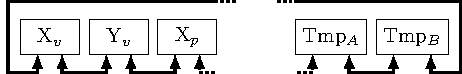
\includegraphics[width=12cm]{geheugen-circ}
		\caption{Circulair registerblok ontwerp en mogelijke operaties\label{figuur-implementatie-miller-geheugen-circ}}
\end{figure}

%TODO: Kansberekening: gemiddeld aantal posities dat x_0 of x_1 van register 1 of 2 verwijderd is.

Omdat de ingangen van de onderliggende schakeling rechtstreeks verbonden zijn met twee registers, is het noodzakelijk om voor elke bewerking de nodige waarden naar die registers over te brengen. Het gemiddeld aantal klokslagen $\overline{t}$ dat daar voor nodig is, kan op de manier die volgt bepaald worden. Eerst wordt de gemiddelde afstand $\overline{r}$ tussen twee variabelen $x_0$ en $x_1$ bepaald. Die is gelijk aan de som $s$ van de mogelijke afstanden $r$ gedeeld door het aantal mogelijke posities $c$ die twee variabelen kunnen bezetten:
\[\begin{aligned}
s	&= \sum_{i = 1}^{n - 1} \sum_{j = i + 1}^n (j - i - 1)
	&\qquad c	&= \sum_{i = 0}^{n - 1} i\\
	&= \frac{n \cdot (n - 1) \cdot (n - 2)}{6}
	&	&= n \cdot \frac{n - 1}{2}\\
\end{aligned}\]
dus
\[\overline{r}	= \frac{n - 2}{3}.\]
Merk op dat deze formules slechts een benadering geven. Zo wordt bijvoorbeeld niet in rekening gebracht dat wanneer beide waarden in de eerste twee registers zitten, er geen doorschuivingen moeten gebeuren.

Per positie die $x_0$ en $x_1$ van elkaar verwijderd zijn, zal een `swap' operatie uitgevoerd moeten. Daartoe dient $x_1$ telkens eerst verplaatst te worden tot register twee. Er zijn dus $\overline{r} \cdot n$ doorschuif operaties nodig. Dit is opnieuw een ruwe schatting, die voor kleine $n$ niet zal kloppen. Algemeen kan echter gesteld worden dat
\[\overline{t} \in \mathcal{O} \Bigl( \frac{n^2}{3} \Bigr).\]

Verder is het energieverbruik recht evenredig met het aantal schrijfbewerkingen die op de registers worden uitgevoerd. Elke doorschuif operatie kost $n$ zulke bewerkingen, m.a.w.\ het gemiddeld aantal schrijfbewerkingen $\overline{w}$ dat uitgevoerd moet worden voor gestart kan worden met de berekening van een optelling of vermenigvuldiging, is
\[\overline{w} \in \mathcal{O} \Bigl( \frac{n^3}{3} \Bigr).\]

Gezien het feit dat er vijftien registers zijn (tegenover zes in \cite{lee}), zou dit zeer veel energie kosten. Verder zou het veel klokslagen in beslag nemen om beide waarden in de correcte registers op te slaan, hoewel zoals eerder bepaald tijdsduur niet van zeer groot belang is. Om dit probleem op te lossen, wordt het mogelijk gemaakt dat elk register ook de waarde van zijn voorganger kan opslaan. Dit is equivalent aan de `swap' (en `copy') operatie toelaten tussen alle aan elkaar grenzende registers. Verder kunnen `swap' operaties tussen twee paar registers in parallel uitgevoerd worden. Uiteraard wordt hiervoor een prijs betaald, er moet nu namelijk per register een extra multiplexer en een selectie signaal voorzien worden.  Het resulterend ontwerp is te zien in \reffig{figuur-implementatie-miller-geheugen-circ-optimized}.

\begin{figure}[h]
	\centering
		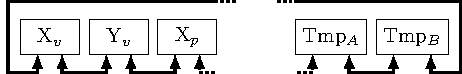
\includegraphics[width=12cm]{geheugen-circ-optimized}
		\caption{Circulair registerblok geoptimaliseerd voor energieverbruik\label{figuur-implementatie-miller-geheugen-circ-optimized}}
\end{figure}

In dit geval zal de afstand $r$ van een waarde $x$ tot het eerste register gelijk zijn aan $\textsf{min}(j - 1, n - j + 1)$ omdat nu in beide richtingen geschoven kan worden. De gemiddelde afstand $\overline{r}$ is dan
\[\begin{aligned}
\overline{r}	&= \frac{1}{n} \cdot \sum_{i = 1}^{n} \textsf{min}(j - 1, n - j + 1)\\
	&= \frac{2}{n} \cdot \sum_{i = 1}^{\frac{n}{2}} (j - 1)\\
	&= \frac{n - 1}{4}.
\end{aligned}\]
Aangezien de omwissel operaties in parallel uitgevoerd kunnen worden, is het gemiddeld aantal klokslagen in dit geval
\[\overline{t} \in \mathcal{O}  \Bigl( \frac{n}{4} \Bigr)\]
en, rekening houdend met het feit dat elke omwissel operatie twee schrijfbewerkingen vraagt en er twee variabelen naar de juiste positie gebracht moeten worden,
\[\overline{w} \in \mathcal{O}(n).\]

Tegenover het originele ontwerp voor het registerblok, zal dit ontwerp veel minder klokslagen verloren laten gaan aan het in de juiste positie brengen van de benodigde variabelen. Ook zal het, ten koste van meer multiplexers, significant minder energie verbruiken. De extra multiplexers zullen echter ook energie vragen, dus in hoeverre dit het totale verbruik naar beneden haalt, moet van implementatie tot implementatie bekeken worden. 

Registers \'e\'en en twee worden respectievelijk met de $A$ en $B$ ingang van de $\mathbb{F}_{2^m}$ kern verbonden. Om vermenigvuldigingen tot een succesvol einde te brengen, moet het register dat met de $A$ ingang verbonden is elke klokslag met $d$ bits naar links doorgeschoven kunnen worden. Hierbij gaat de originele waarde van het register echter wel verloren. Wanneer de algoritmes die het meeste tijdelijke opslag vragen echter nauwkeurig worden bekeken, zal men merken dat dit geen probleem vormt. Vandaar dat er voor gekozen wordt om het derde tijdelijk register uit de doorschuif lus te halen, er moeten dan minder doorschuivingen doorgevoerd worden om elke waarde in de juiste positie te brengen. Verder moet het ook mogelijk zijn waarden die op de ingang van de Miller controller aangelegd worden op te slaan en het resultaat op de uitgang te zetten. Ten slotte moet het resultaat van een berekening in $\mathbb{F}_{2^m}$ opgeslagen kunnen worden. Teneinde dat mogelijk te maken, wordt de uitgang $R$ van de $\mathbb{F}_{2^m}$ kern aan het derde tijdelijk register gekoppeld. Rekend houdend met deze zaken, wordt het ontwerp van de eerste twee registers aangepast zoals te zien in \reffig{figuur-implementatie-geheugen-eerste-twee}.

\begin{figure}[h]
	\centering
		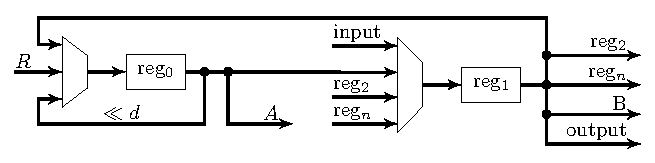
\includegraphics[width=12cm]{geheugen-eerste-twee}
		\caption{Ontwerp van de schakeling rond de eerste twee registers in het registerblok\label{figuur-implementatie-geheugen-eerste-twee}}
\end{figure}

\subsection{FSM}

Met alle details over de hardware bekend, kan overgegaan worden tot het ontwerp van een FSM. Daarbij zullen een zeer groot deel van de te implementeren states niets anders doen dan geheugen verschuifen. Om het geheel overzichtelijk te houden, zal het ontwerp dan ook niet tot op state niveau gebeuren. Ook zal zoveel mogelijk getracht worden reeds ge\"implementeerde states opnieuw te gebruiken.

Aangezien een beeld meer zegt dan duizend woorden, wordt het resultaat zonder veel extra uitleg gepresenteerd in \reffig{figuur-miller-fsm}. Wat wel enige extra aandacht verdient, is de opsplitsing van de verdubbel- en optelstap. Wanneer \refalg{algoritme-implementatie-miller-double-detail} en \ref{algoritme-implementatie-miller-add-detail} opnieuw bekeken worden, valt het op dat buiten de berekening van $\lambda$ en het nieuwe $x$-co\"ordinaat van $V$ alle andere berekeningen zeer gelijkaardig zijn. Meer nog, indien de paren $(x_V, y_V)$ en $(x_P, y_P)$ vervangen worden door een algemene $(x_A, y_A)$, dan bestaan beide algoritmes uit dezelfde bewerkingen na het berekenen van $\lambda$ en $x_V$. Aangezien na de berekening van $\lambda$ nog steeds twee registers vrij zijn voor gebruik, kunnen deze aangewend worden om de toepasselijke $x$ en $y$ co\"ordinaten in op te slaan. Op die manier kunnen de verdere berekeningen met dezelfde states uitgewerkt worden, ongeacht of nu de verdubbel- of de optelstap uitgevoerd wordt.

\begin{figure}[h]
	\centering
		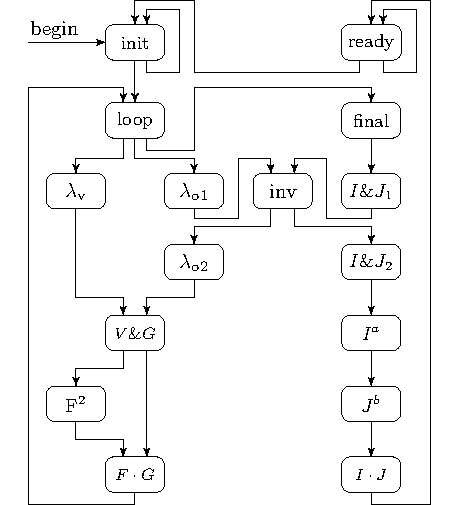
\includegraphics[width=12cm]{miller-fsm}
		\caption{FSM ontwerp van de controller voor het Miller algoritme\label{figuur-miller-fsm}}
\end{figure}

\section{Optimalisaties\label{sectie-implementatie-optimalisaties}}

Nu de schakeling volledig ontworpen is, kan overgegaan worden tot optimalisering. Daarbij wordt opnieuw op de eerste plaats getracht de oppervlakte kleiner te maken, maar er zal ook aandacht gegeven worden aan het beperken van het energieverbruik van de schakeling. De optimalisaties die in de volgende paragrafen voorgesteld worden, zullen allemaal iets te maken hebben met de registers. Omdat de enkele registers van grootte $1$ of $\textsf{log}_2(m)$ bit niet veel bijdragen aan zowel de uiteindelijke oppervlakte als het verbruik zullen de optimalisaties specifiek gericht zijn op het effici\"enter maken van het geheugenblok in de controller voor de Miller loop.

Een register is doorgaans opgebouwd uit een hoeveelheid D-type master-slave flip-flops. Dit type flip-flops slaat de waarde aan de ingang $D$ op bij een stijgende klokslag op ingang $CLK$ en toont deze waarde aan de uitgang $Q$ vanaf de daaropvolgende neergaande klokslag. In alle paragrafen die volgen, wordt er van uit gegaan dat alle registers uit dit type flip-flops opgebouwd zijn.

\subsection{Registers zonder reset}

Een makkelijke eerste aanpassing is het verwijderen van de reset ingangen van de registers. Zoals reeds gezien in \reftbl{tabel-implementatie-beperkingen-elementen-gatecount} kost een D flip-flop zonder reset ingang 0.5 gates minder per bit dan \'e\'en met, een verkleining van $8.5\%$. In het geval van $m = 163$ kijkt men dan aan tegen een besparing van $978 - 896.5 = 81.5$ gates per register. Merk echter wel op dat ten minste \'e\'en register moet overblijven dat wel op 0 (en 1) ingesteld kan worden, om $F$ in te stellen aan het begin van het algoritme.

\subsection{Clock gating\label{subsectie-implementatie-optimalisatie-clock-gating}}

%TODO: Is this correct? The thing about losing multiplexers, etc.

Normaal wordt een register elke klokslag immers geladen met de waarde aan zijn ingang en is het dus noodzakelijk het register naar zichzelf terug te koppelen, wil men geen data verliezen. Een voor de hand liggende techniek, clock gating, laat toe deze terugkoppeling (en de daarbij horende multiplexer) achterwege te laten. Bij deze techniek wordt het kloksignaal enkel gepropageerd naar een register wanneer een daarbij horende enable ingang hoog is. Het implementeren van clock gating kost enige extra oppervlakte. Per register moet echter slechts \'e\'en bijhorende clock gating schakeling voorzien  worden en de schakelingen zijn zeer klein zijn. Netto zal er dus nog steeds oppervlakte winst gemaakt worden door de eliminatie van de multiplexers.

De eenvoudigste schakeling waarmee clock gating ge\"implementeerd kan worden is te zien in \reffig{figuur-implementatie-optimalisatie-cg-basic}. Er zijn echter enkele problemen geassocieerd met dit type schakeling. Ze is immers onderhevig aan glitches op het enable signaal. Stel bijvoorbeeld dat de enable ingang al hoog wordt terwijl het kloksignaal ook nog hoog is. Dan zal het kloksignaal gepropageerd worden tot het register, wat niet de bedoeling is.

\begin{figure}[h]
	\centering
		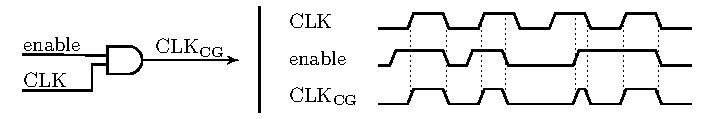
\includegraphics[width=12cm]{cg-basic}
		\caption{Schakeling voor clock gating - Basis ontwerp\label{figuur-implementatie-optimalisatie-cg-basic}}
\end{figure}

Dit probleem kan overkomen worden met de schakeling voorgesteld in \reffig{figuur-implementatie-optimalisatie-cg-no-glitch}. De D latch zorgt er hier voor dat het enable signaal pas wordt doorgelaten nadat het kloksignaal laag geweest is. Hierdoor worden mogelijke glitches dus tegengehouden voor de ze klokingang van het register kunnen bereiken.

\begin{figure}[h]
	\centering
		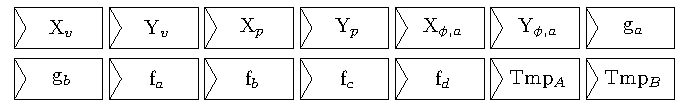
\includegraphics[width=12cm]{cg-no-glitch}
		\caption{Schakeling voor clock gating - Glitchvrij ontwerp\label{figuur-implementatie-optimalisatie-cg-no-glitch}}
\end{figure}

Ten slotte is er een derde oplossing die toelaat een nog grotere energiebesparing door te voeren, zoals aangetoond in \cite{mueller}. In die paper wordt aangetoond dat het energie verbruik van een D-type master-slave flip-flop veel hoger is wanneer het kloksignaal laag is, dan wanneer het hoog is. De reden hiervan is duidelijk te zien in \reffig{figuur-implementatie-optimalisatie-cg-power-dis}: wanneer de klok laag is, veranderen telkens de ingang verandert twee interne poorten van staat en wijzigen de gate capaciteiten van twee andere poorten. Indien de klokingang hoog is, wijzigt een veranderend ingangssignaal enkel de gate capaciteit van de eerste interne poort.

\begin{figure}[h]
	\centering
		\subfigure[$CLK = 0$]{
			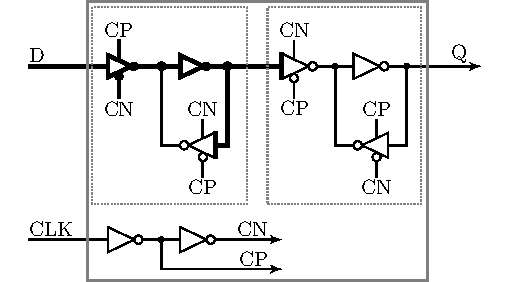
\includegraphics[width=5.7cm]{cg-pow-dis-zero}
			%\label{subfig-1-implementatie-optimalisatie-cg-power-dis}
		}
		\subfigure[$CLK = 1$]{
			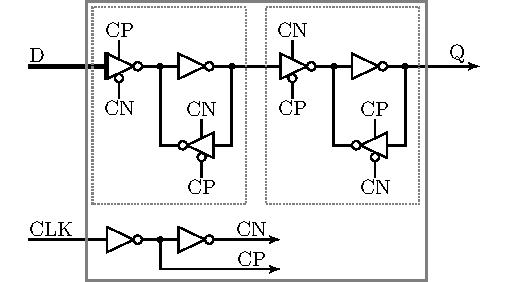
\includegraphics[width=5.7cm]{cg-pow-dis-one}
			%\label{subfig-2-implementatie-optimalisatie-cg-power-dis}
		}
		\caption[Stroomverbruikende componenten van een D-type master-slave flip-flop bij constante waarde van de klok ingang]{Stroomverbruikende componenten van een D-type master-slave flip-flop bij constante waarde van de klok ingang \protect\cite{mueller}\label{figuur-implementatie-optimalisatie-cg-power-dis}}
\end{figure}

Helaas is de werking van de twee vorige schakelingen net zo dat de klokingang laag gehouden wordt zolang de enable ingang laag is. De oplossing ligt in de schakeling in \reffig{figuur-implementatie-optimalisatie-cg-low-power}, die exact doet wat nodig is: de klokingang hoog houden zolang geen nieuwe waarde in het register opgeslagen moet worden. Om het voorkomen van glitches te garanderen, moet het enable signaal stabiel worden voor het CLK signaal hoog wordt. Indien bepaalde kloksignaalbeperkingen worden opgelegd bij het synthetiseren van het circuit is dit normaal gezien echter geen probleem.

\begin{figure}[h]
	\centering
		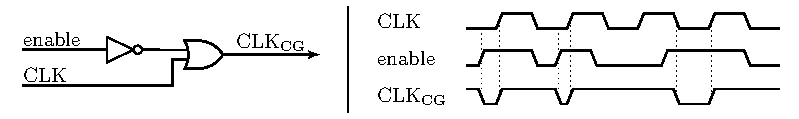
\includegraphics[width=12cm]{cg-low-power}
		\caption{Schakeling voor clock gating - Laag vermogen ontwerp\label{figuur-implementatie-optimalisatie-cg-low-power}}
\end{figure}
